\section{Laser 635\,nm}
\begin{table}
\begin{center}
\caption{ Wyznaczone wartośc prądu progowego $I_{\mathrm{th}}$ w różnych temperaturach $T$ dla lasera krawędziowego 635\,nm. }
\begin{tabular}{ | C{1.5cm}|  C{1.5cm} | C{1.5cm} | C{1.5cm}| C{1.5cm} | C{1.5cm}| C{1.5cm}| C{2.0cm}| C{2.0cm}|}
\hline
$T$ [K] 	&   278 & 283  	& 288 & 293 & 298 & 303 & 308 \\ \hline
$I_{\mathrm{th}}$ [mA]  &	19.1 $\pm$ 0.2  & 20.7 $\pm$ 0.2 & 22.6 $\pm$ 0.2 &
25.0 $\pm$ 0.2  & 27.9 $\pm$ 0.3 & 31.4 $\pm$ 0.5 & 36 $\pm$ 2	\\ \hline
\end{tabular}
\end{center}
\end{table}
%\begin{figure}
%\center
%  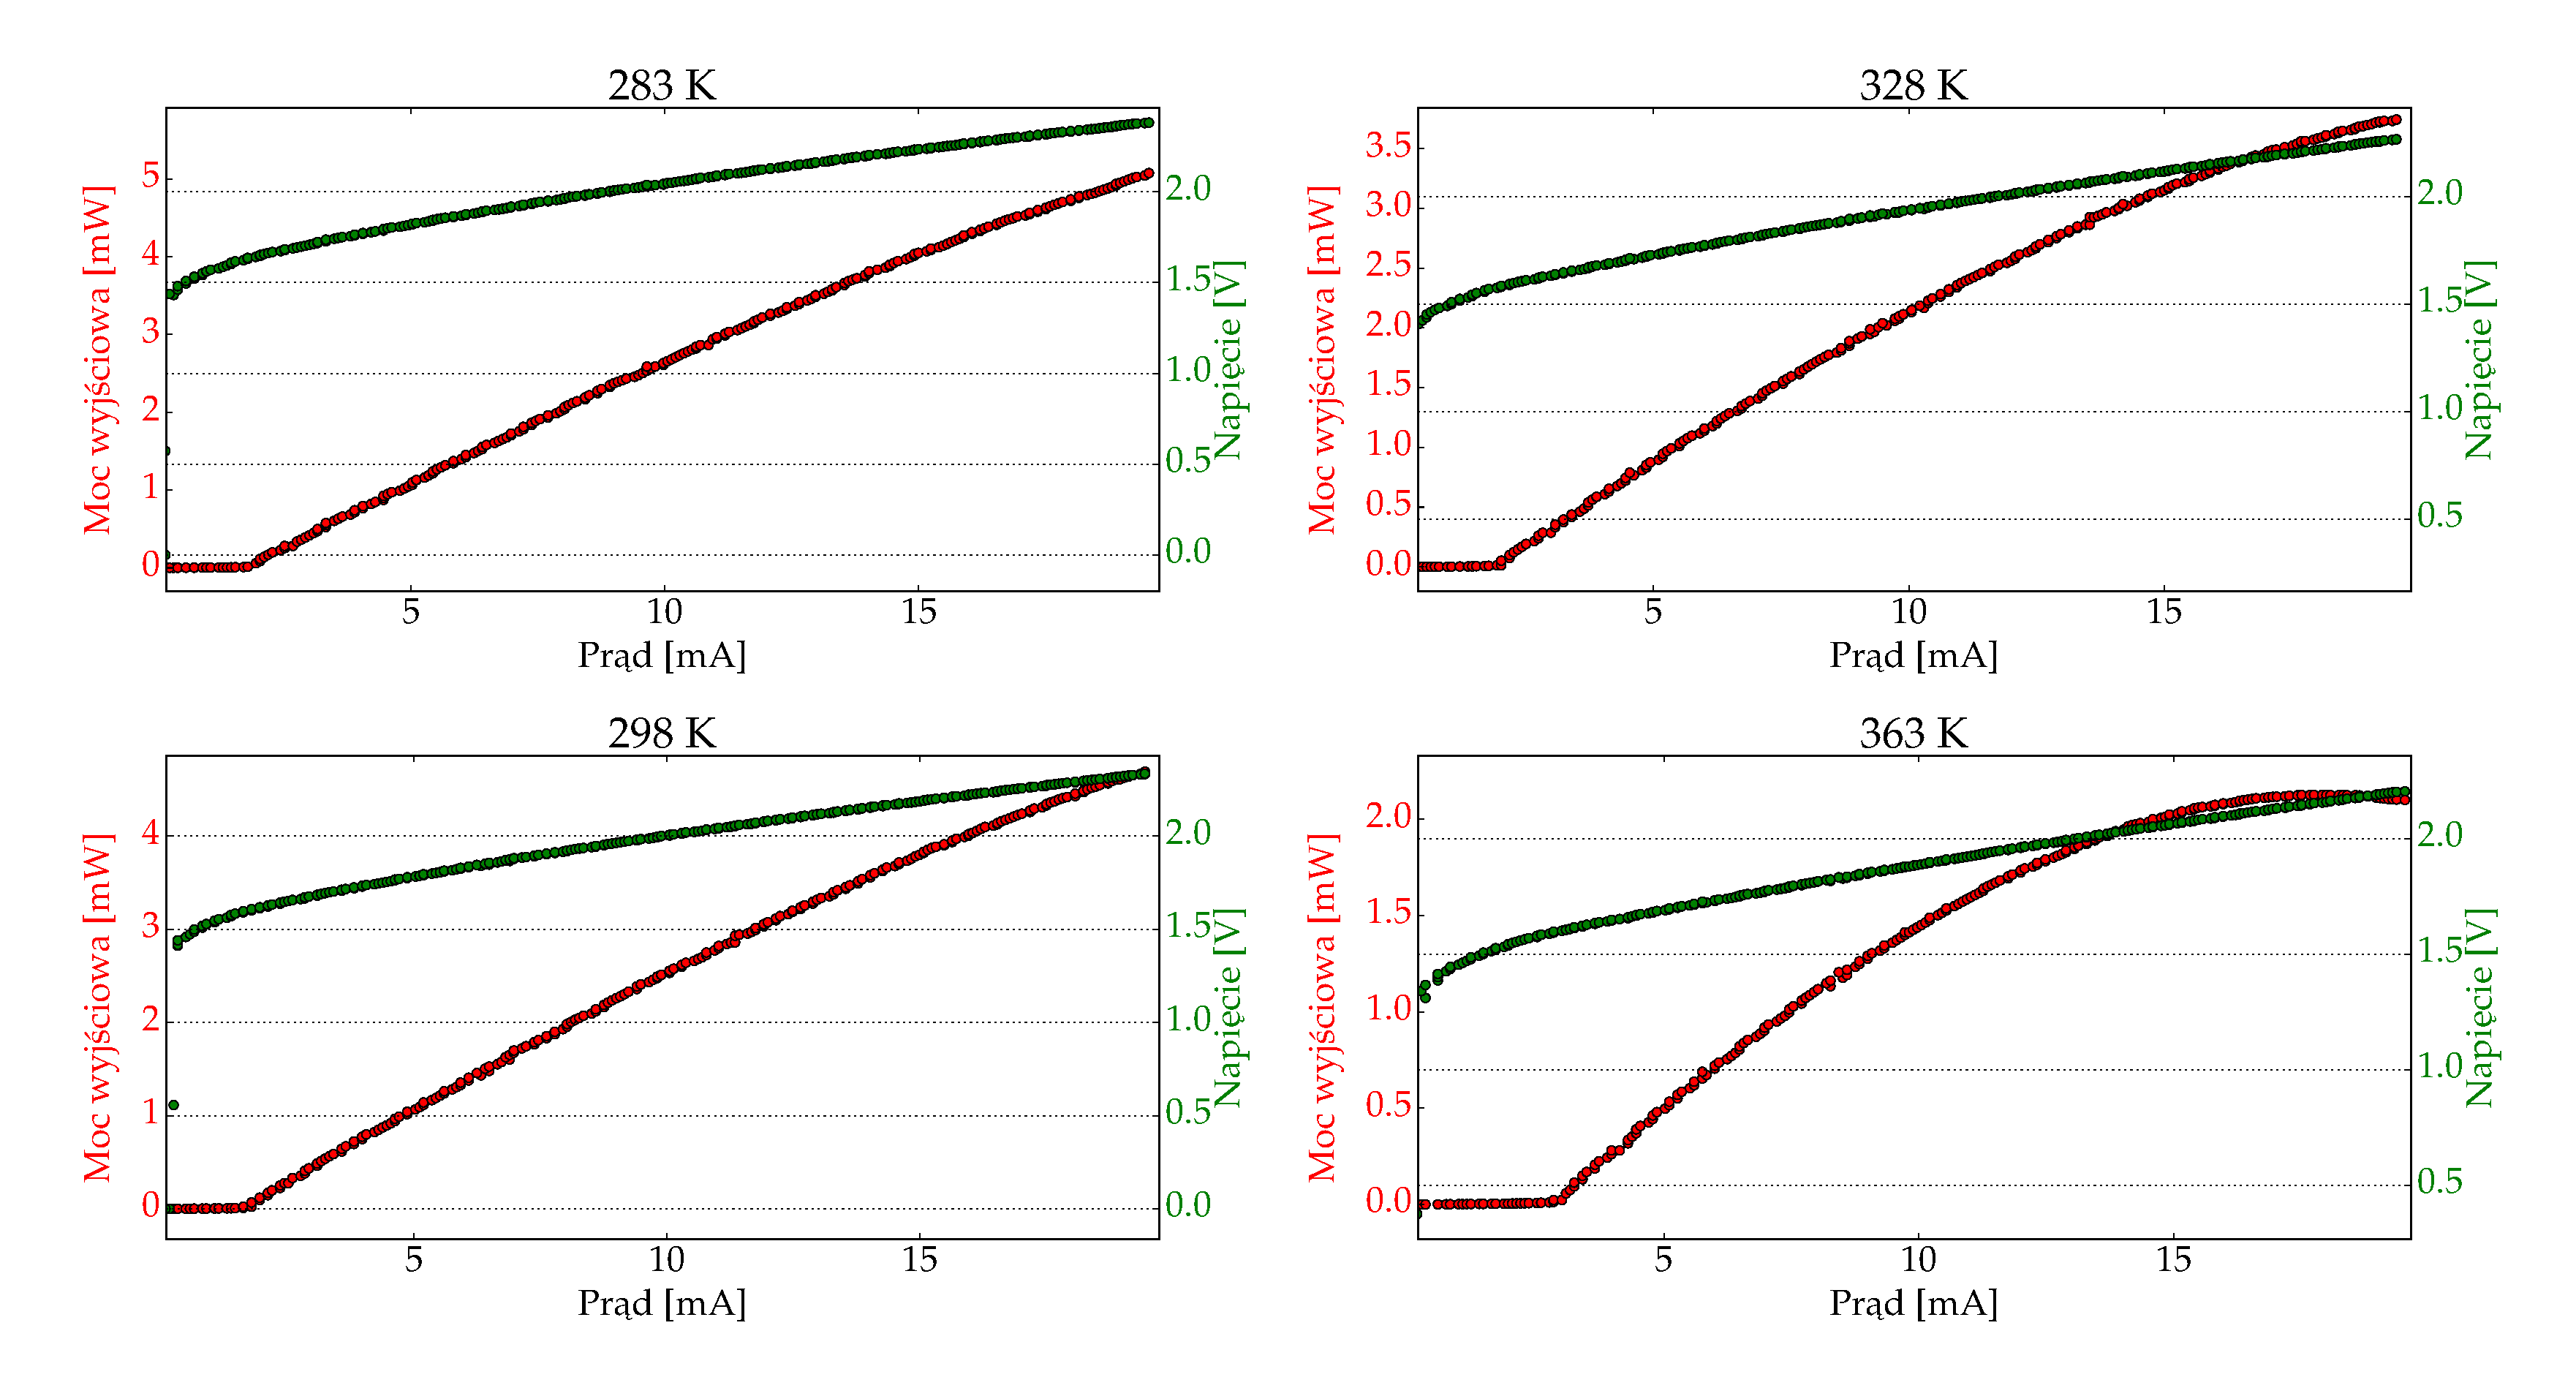
\includegraphics[scale=0.30]{plot635/plot_ivl_4.eps}
%  \label{rys1}
%  \caption{Wykres napięcia i mocy od prądu dla lasera krawędziowego 635\,nm.}
%\end{figure}
\begin{figure}
\center
  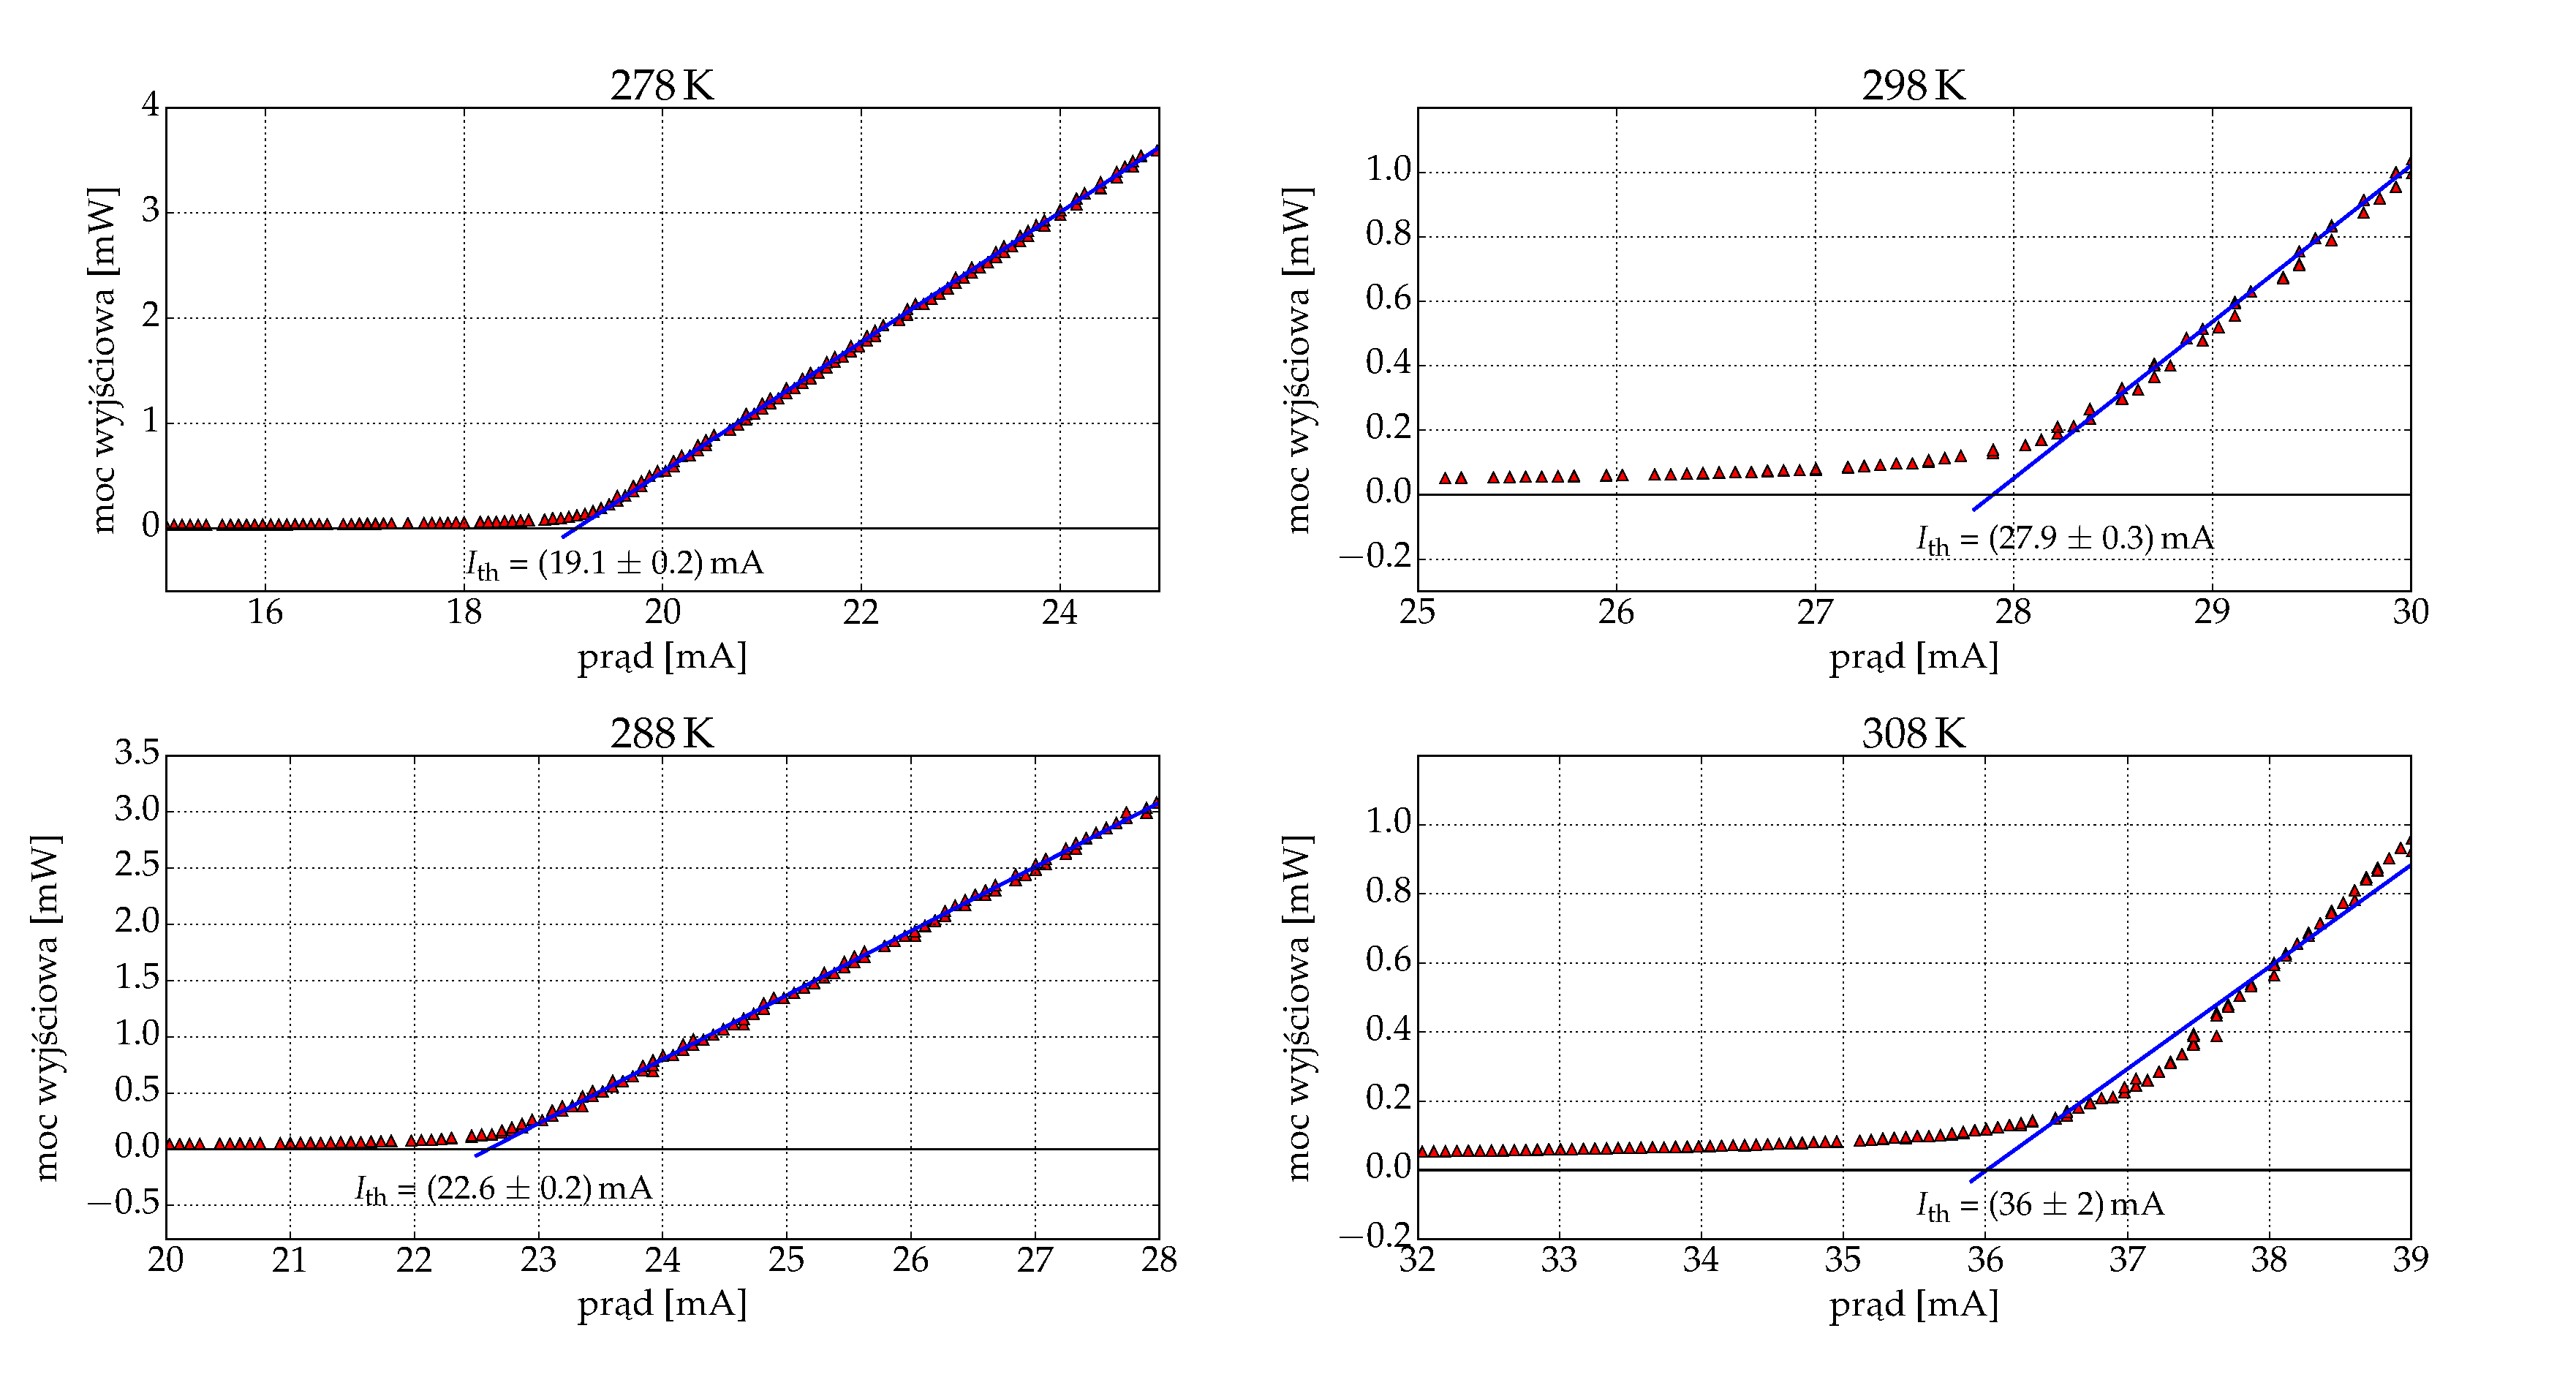
\includegraphics[scale=0.30]{plot635/plot_i_th_4.eps}
  \label{rys2}
  \caption{Wykres prądu progowego dla lasera krawędziowego 635\,nm.}
\end{figure}
\begin{figure}
\center
  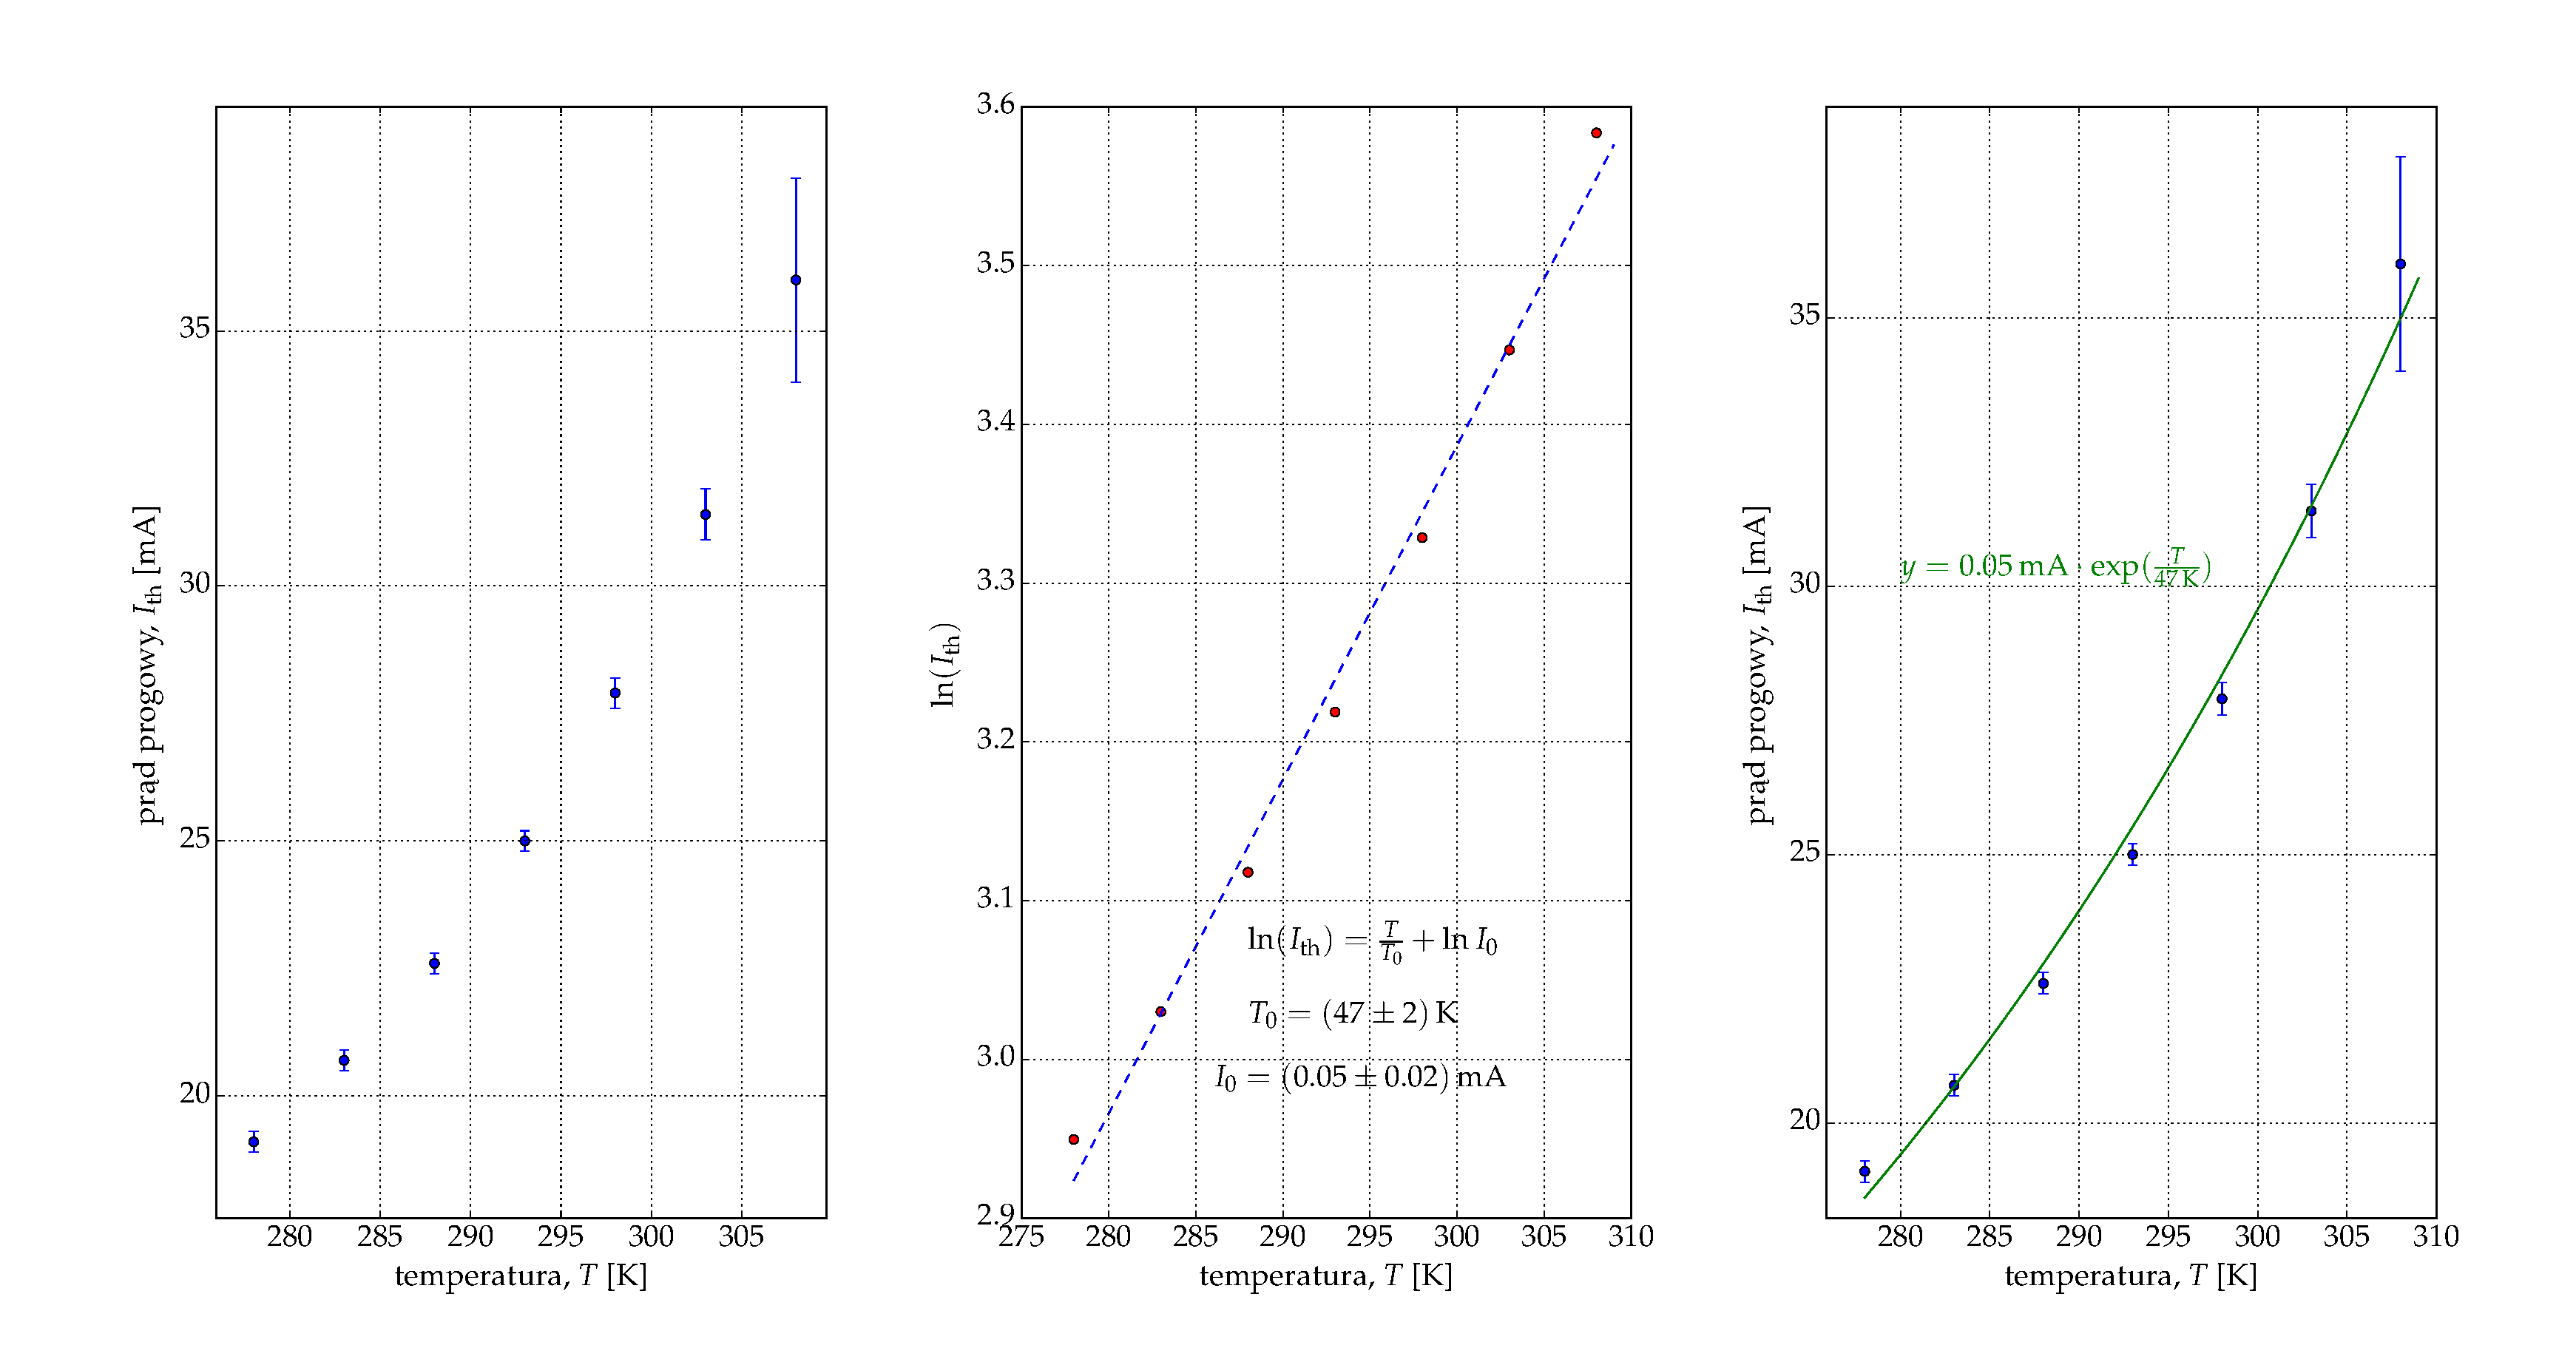
\includegraphics[scale=0.30]{plot635/plot_fit.eps}
  \label{rys2}
  \caption{Wykres prądu progowego z dopasowanymi wartościami $I_{0}$ i $T_{0}$ dla lasera krawędziowego 635\,nm.}
\end{figure}
\begin{figure}
\center
  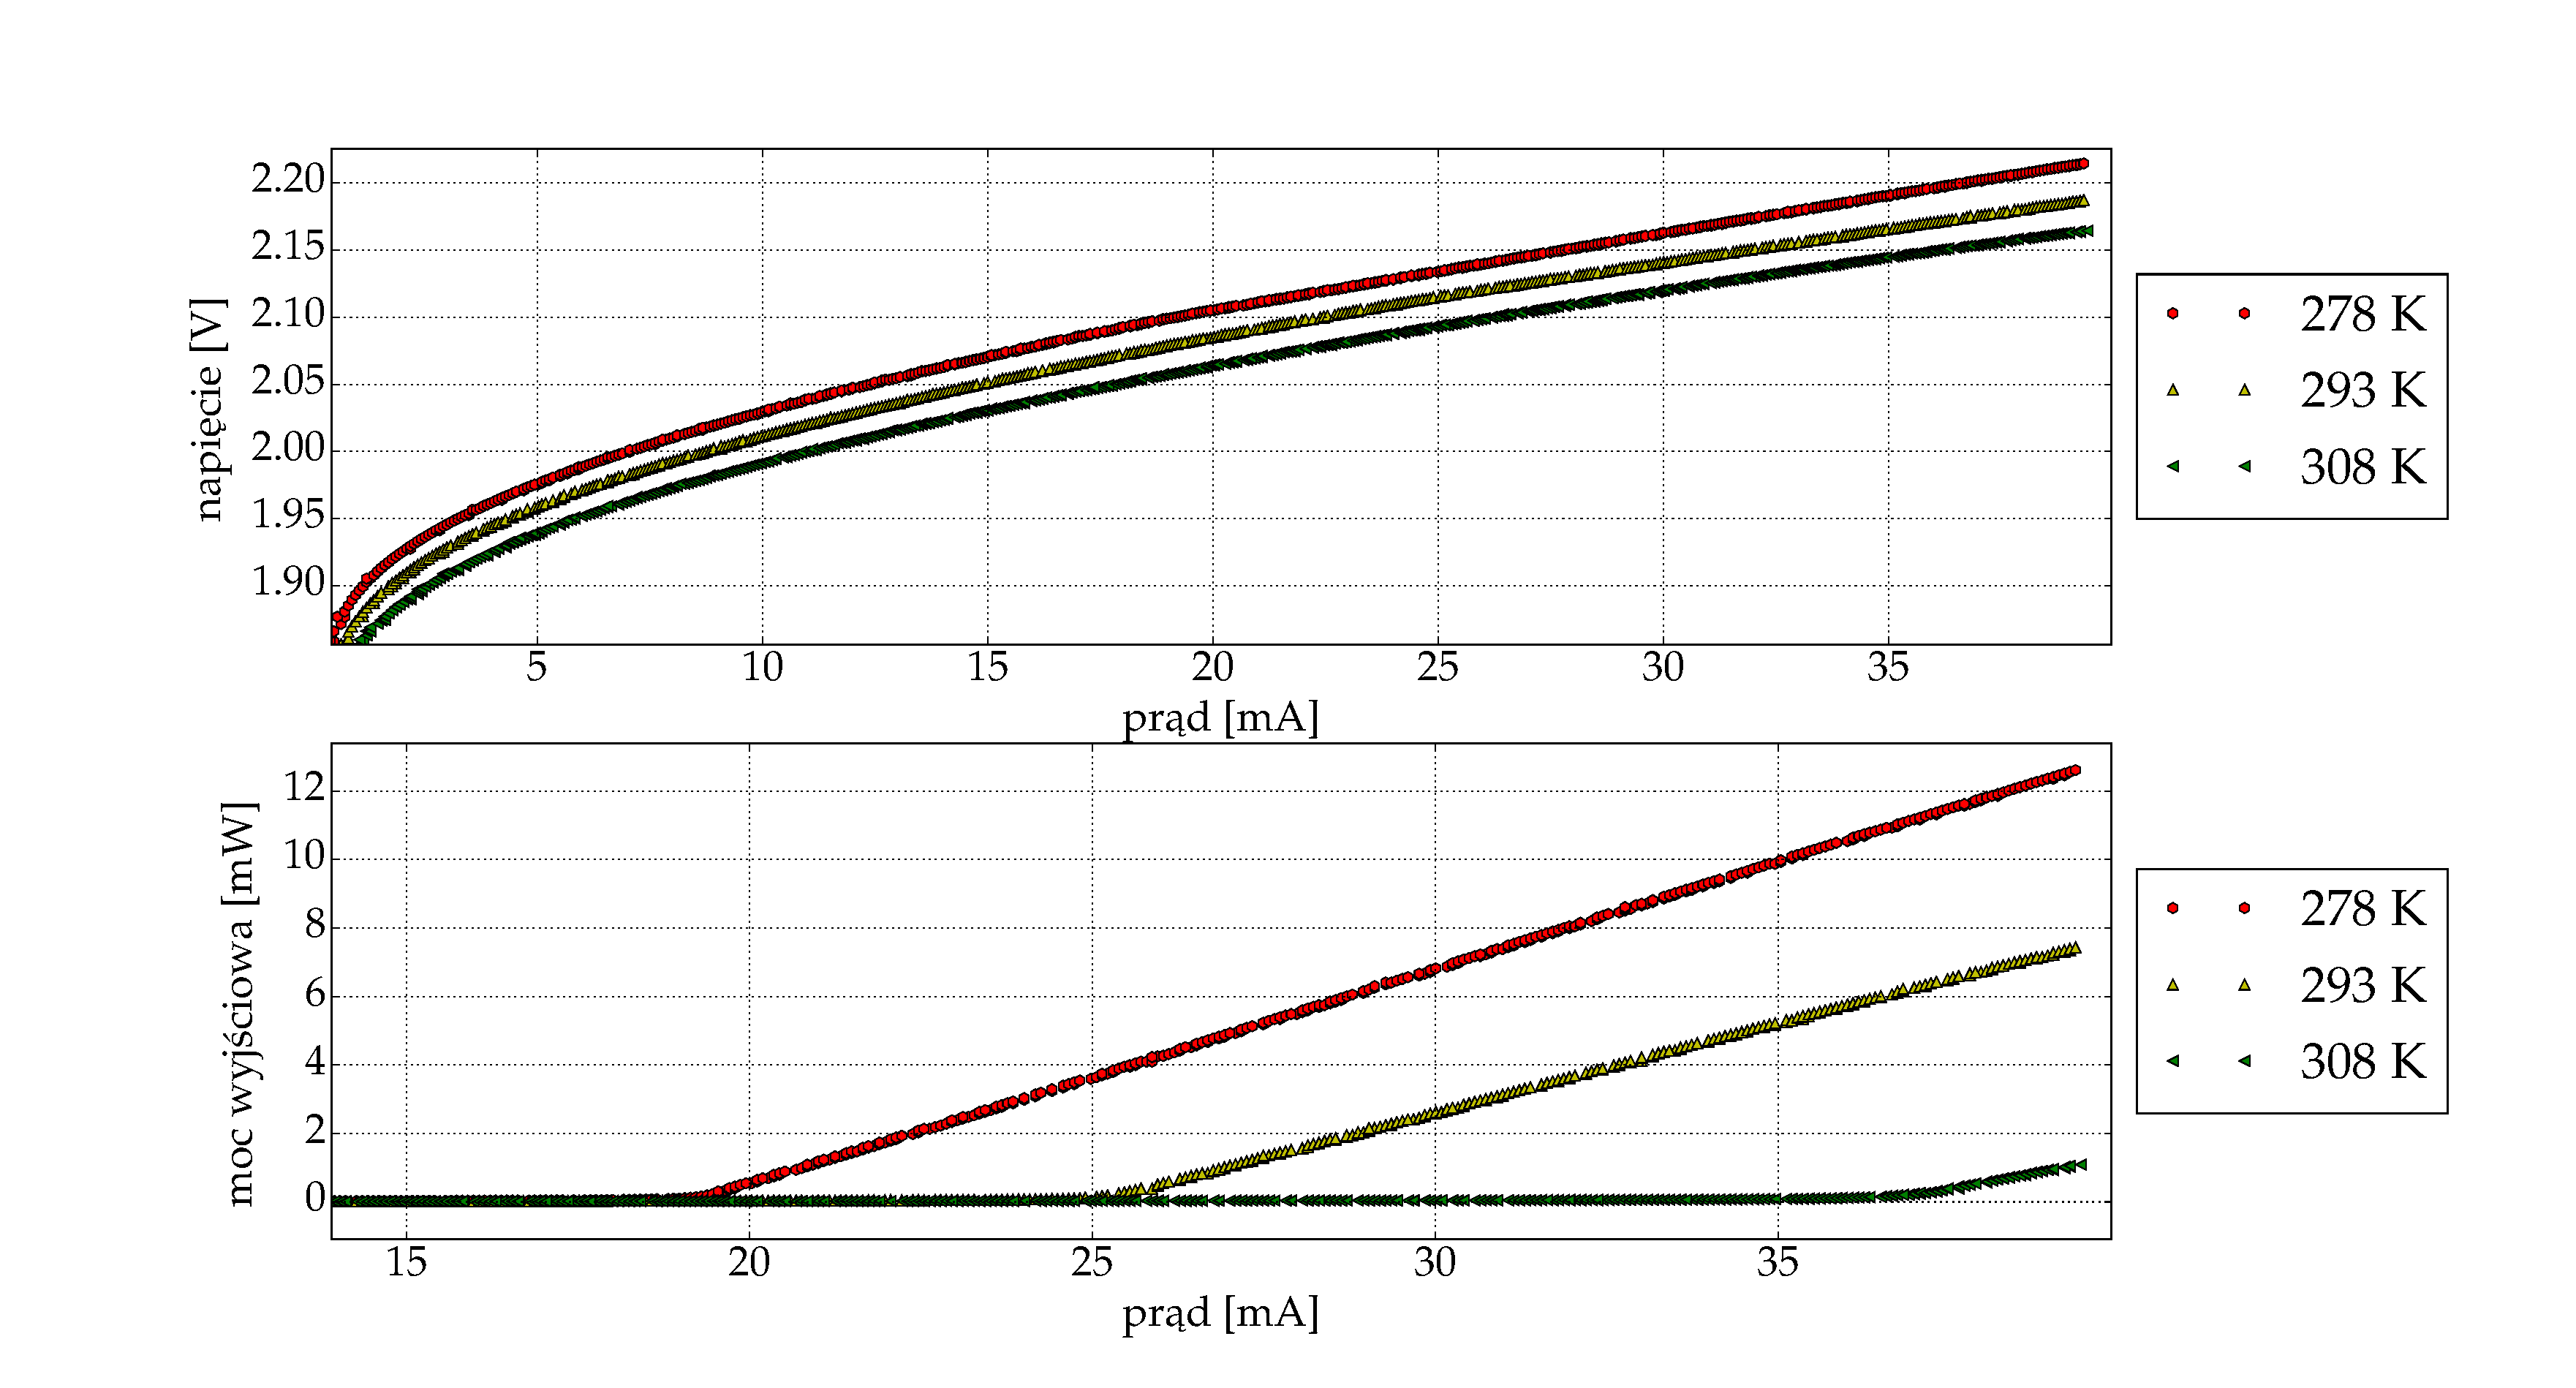
\includegraphics[scale=0.30]{plot635/plot_voltage_power.eps}
  \label{rys3}
  \caption{Wykres napięcia na laserze oraz mocy w funkcji prądu dla lasera krawędziowego 635\,nm.}
\end{figure}
\begin{figure}
\center
  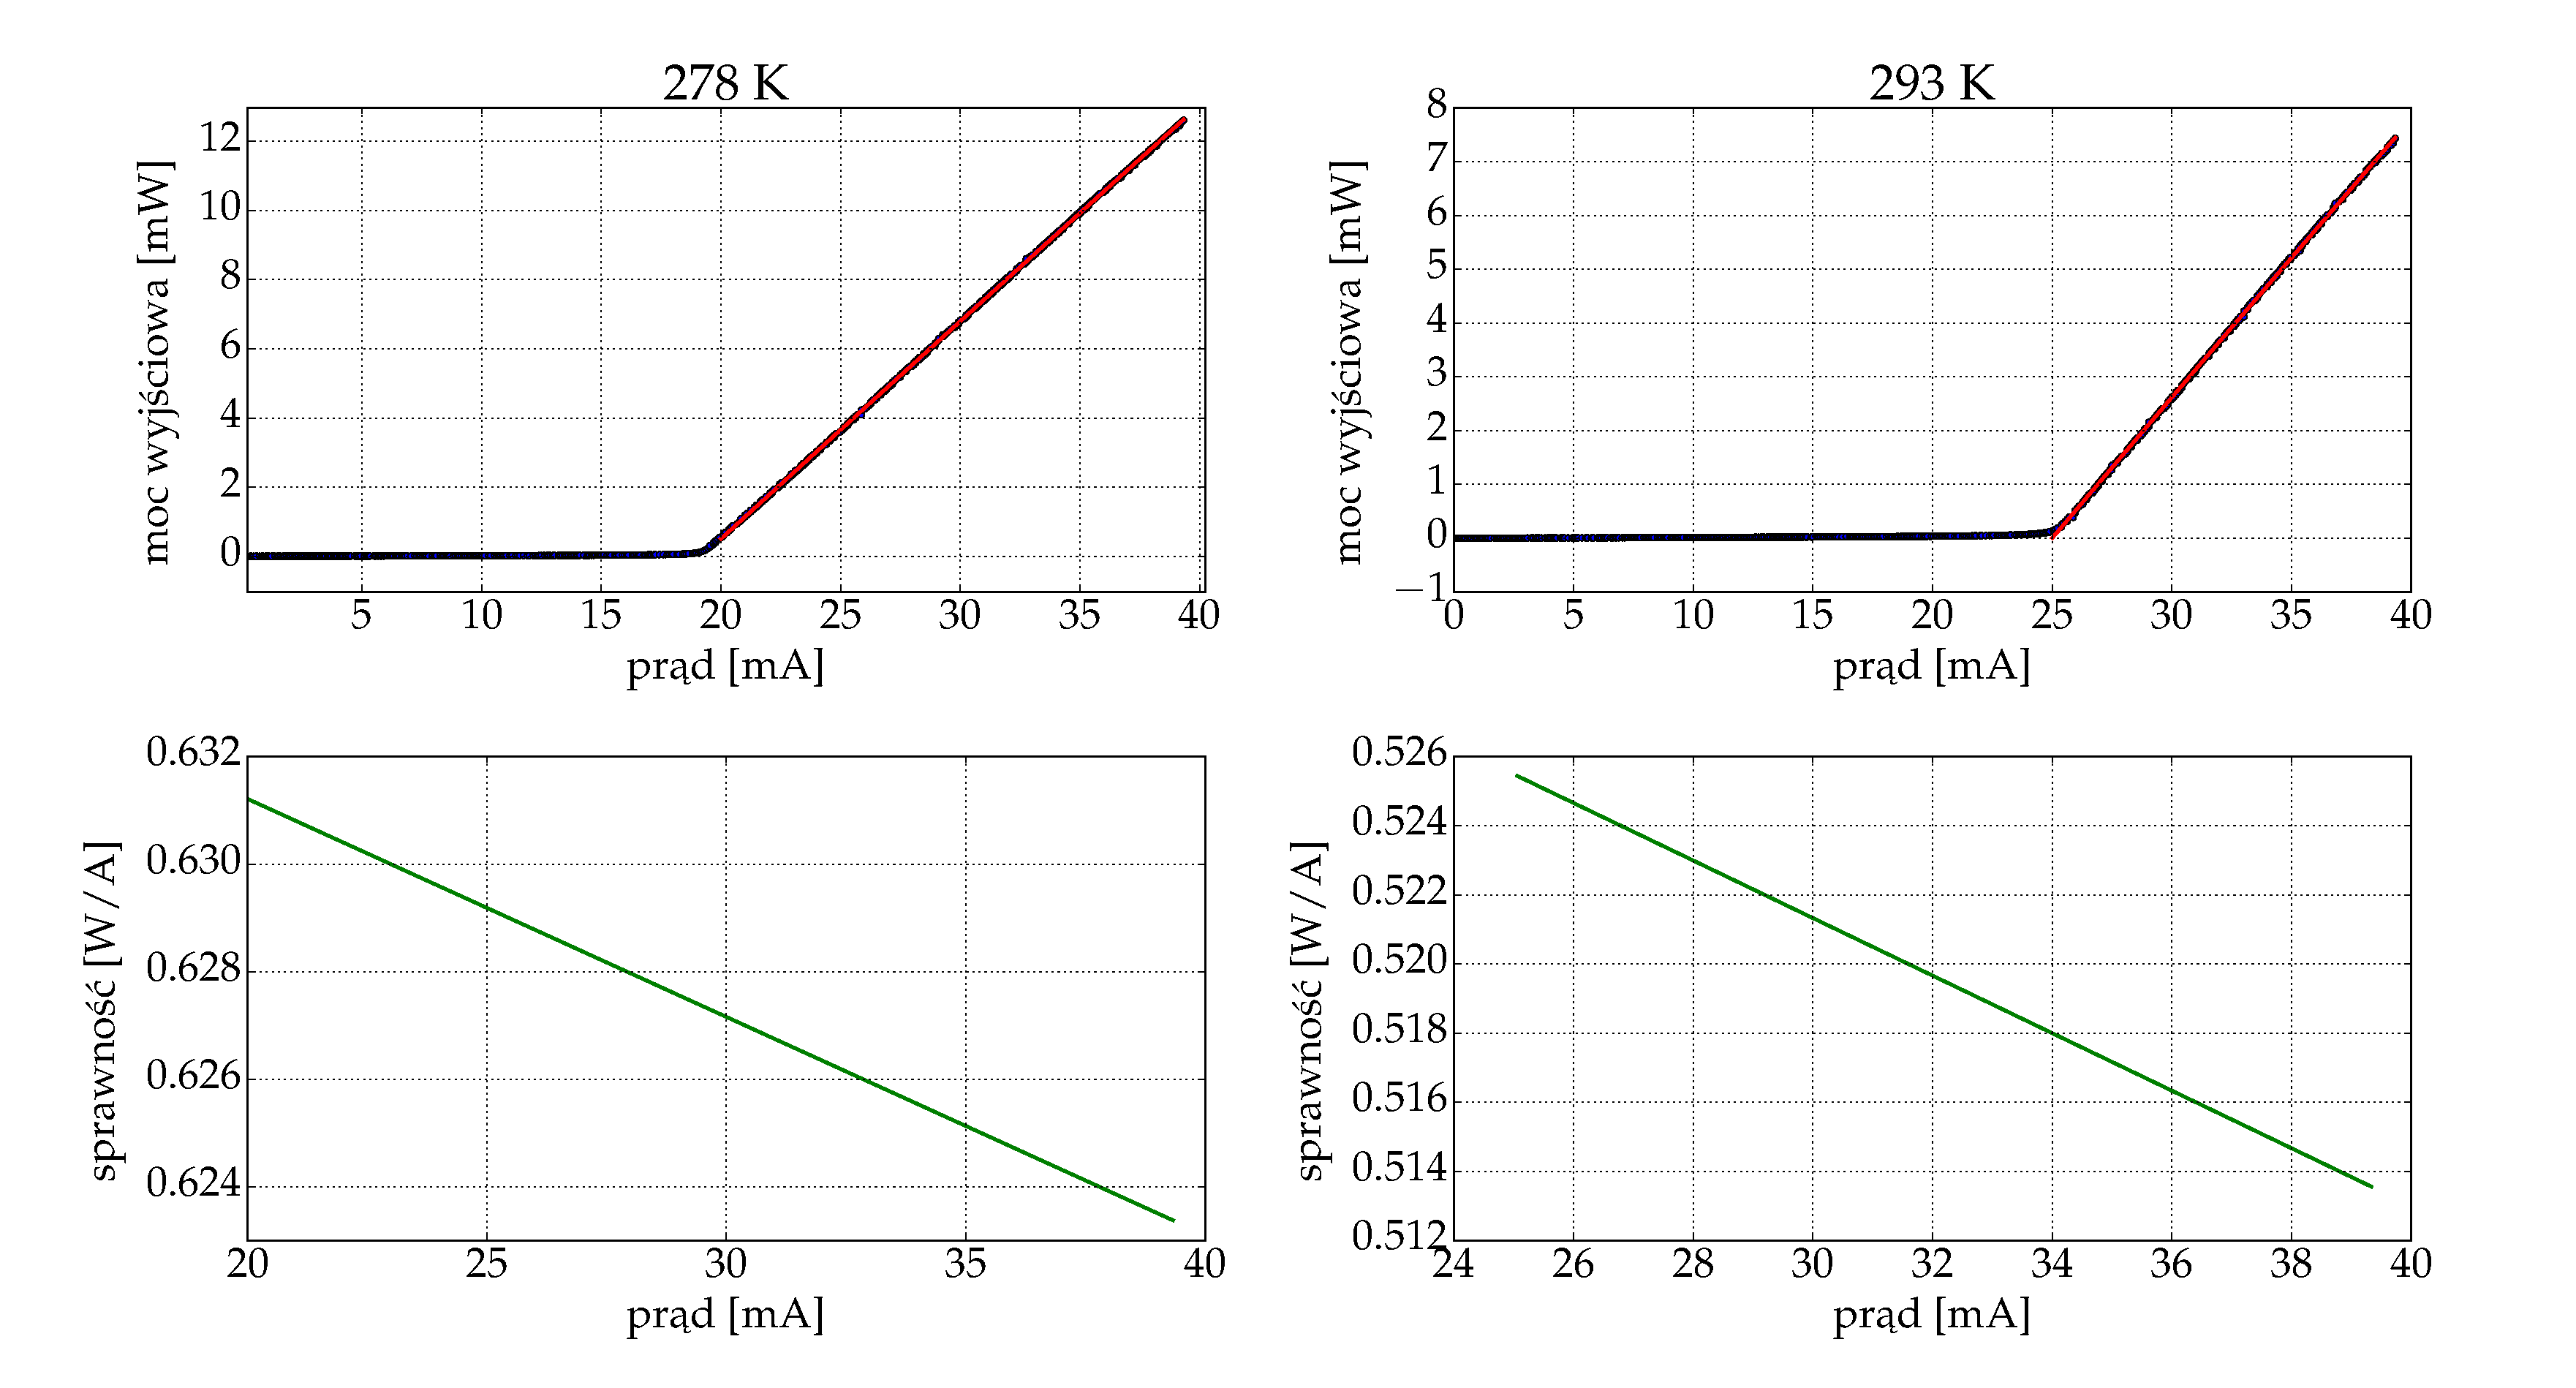
\includegraphics[scale=0.30]{plot635/plot_eff_via_current4.eps}
  \label{rys3}
  \caption{Wykres sprawności różniczkowej dla lasera krawędziowego 635\,nm dla dwóch temperatur.}
\end{figure}
\begin{figure}
\center
  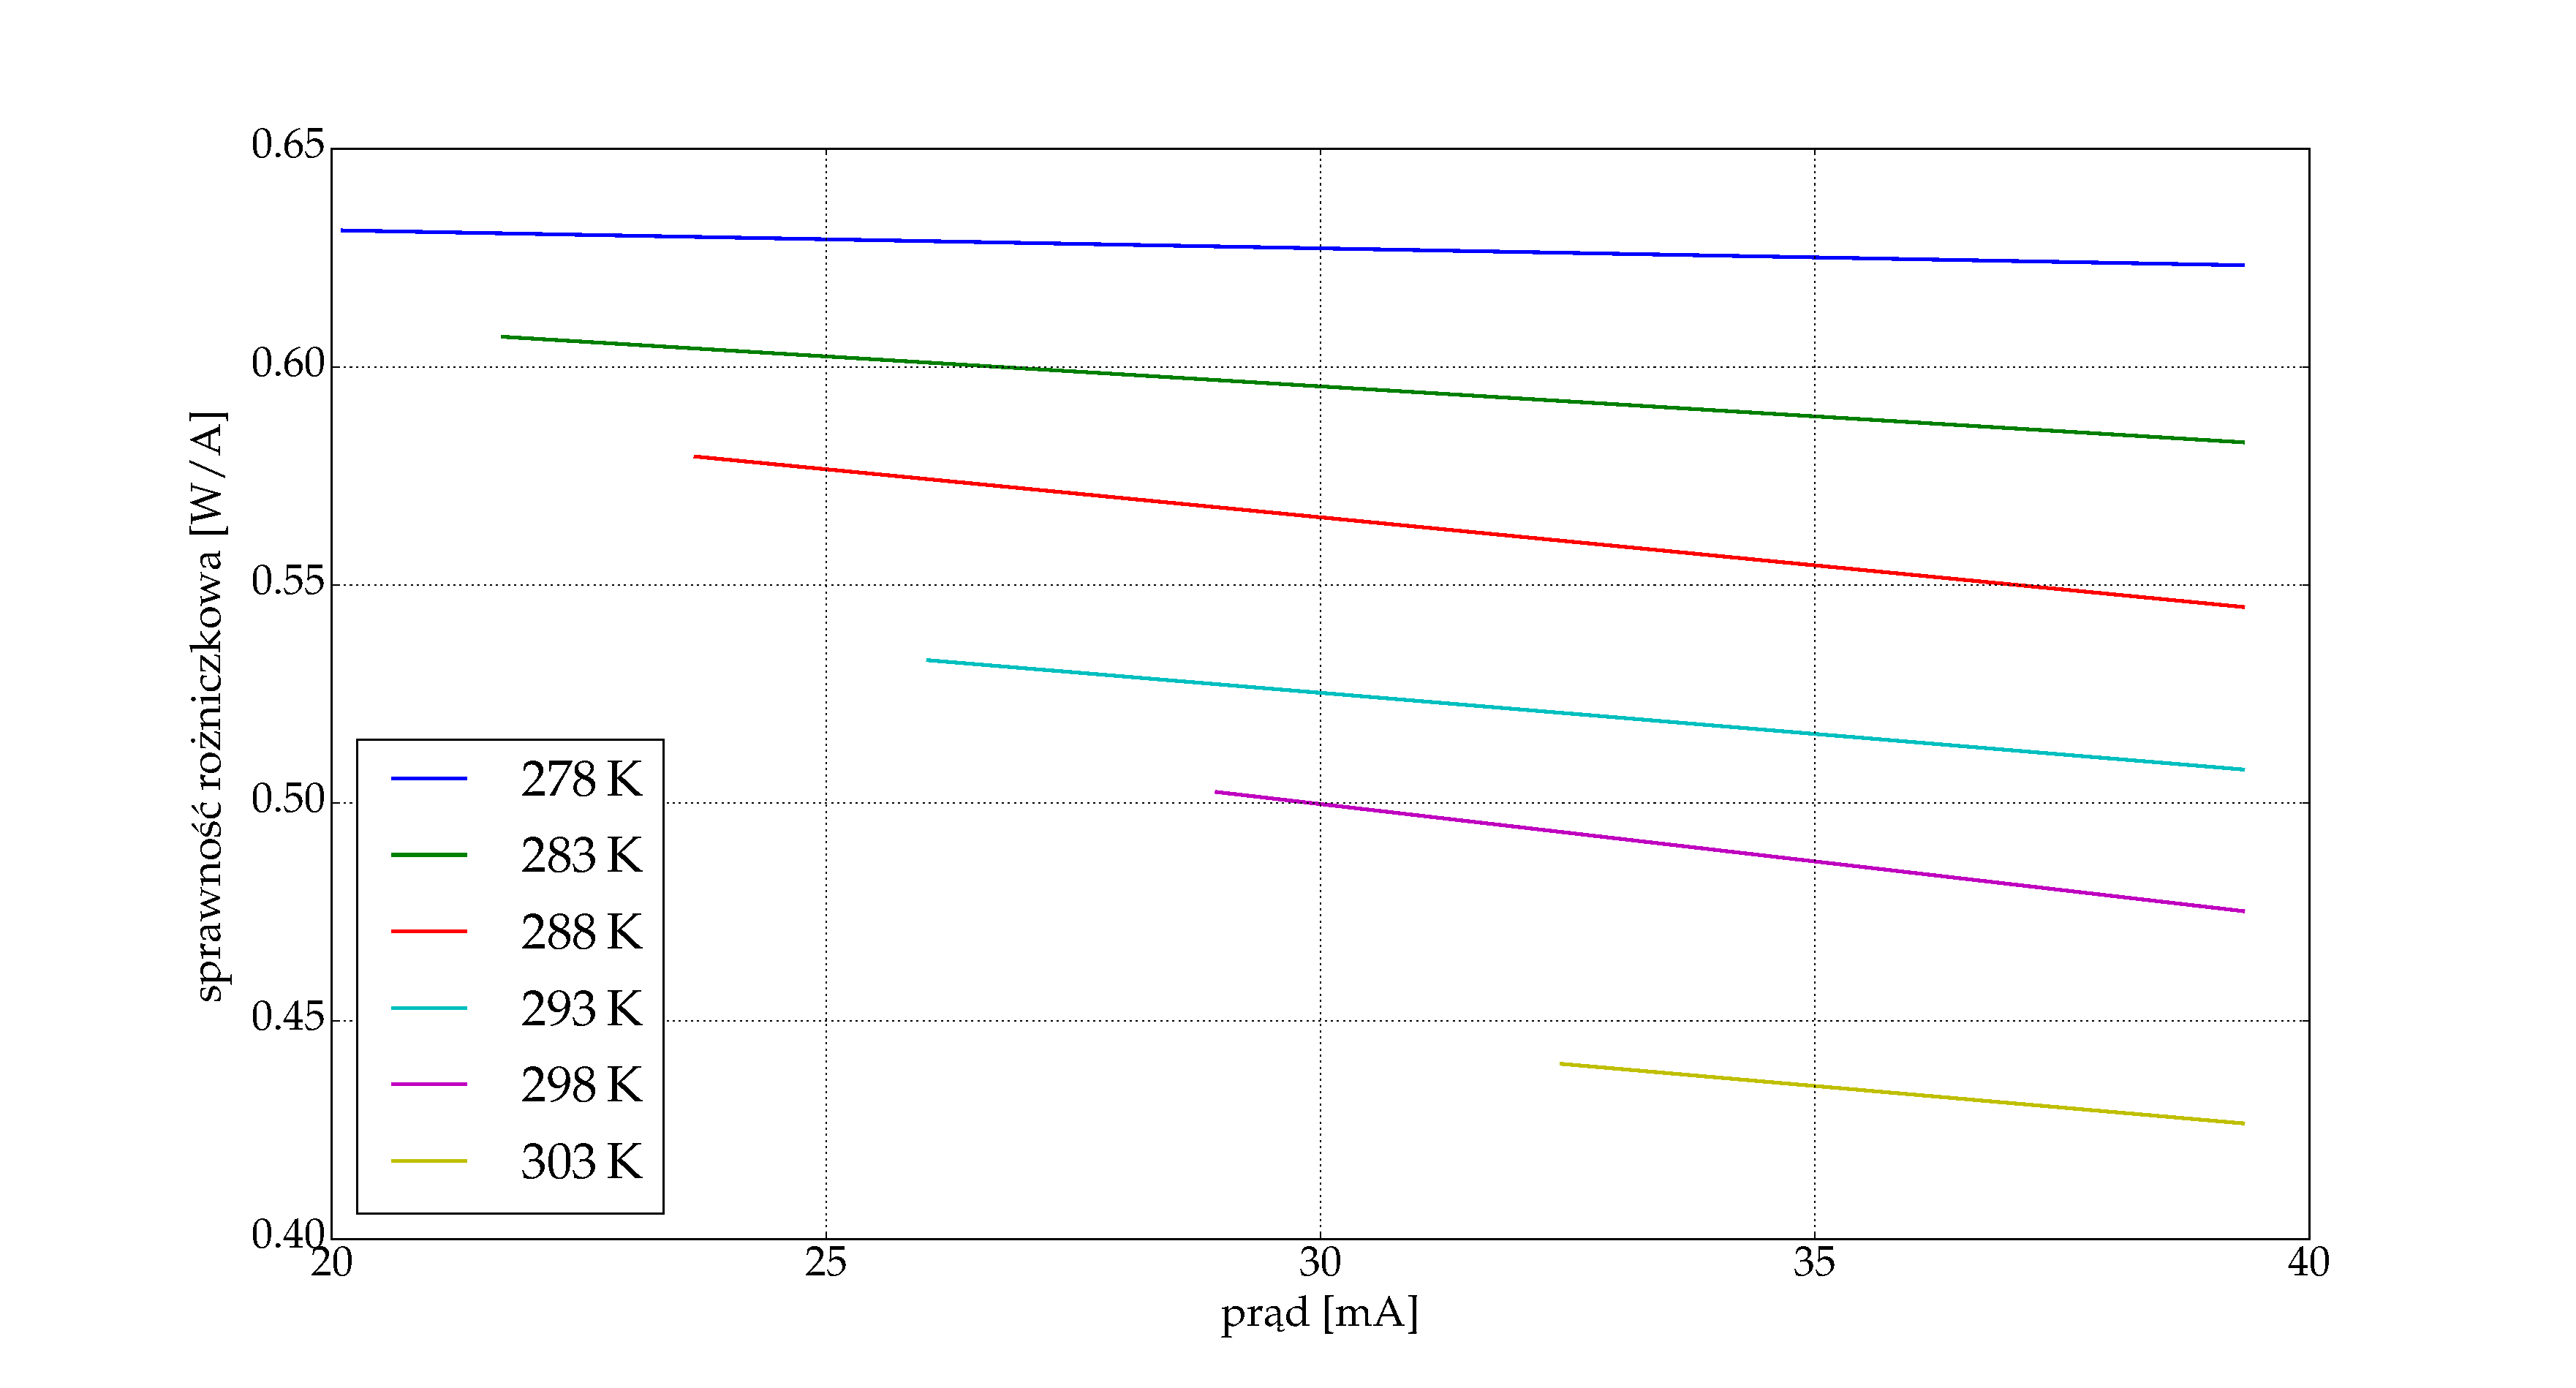
\includegraphics[scale=0.30]{plot635/plot_eff_via_current_all.eps}
  \label{rys3}
  \caption{Wykres sprawności w funkcji prądu dla lasera krawędziowego 635\,nm.}
\end{figure}